\documentclass[letterpaper,10pt]{article}

\usepackage{titling}
\usepackage{listings}
\usepackage{url}
\usepackage{setspace}
\usepackage{subfig}
\usepackage{sectsty}
\usepackage{pdfpages}
\usepackage{colortbl}
\usepackage{multirow}
\usepackage{multicol}
\usepackage{relsize}
\usepackage{amsmath}
\usepackage{fancyvrb}
\usepackage{amsmath,amssymb,amsthm,graphicx,xspace}
\usepackage[titlenotnumbered,noend,noline]{algorithm2e}
\usepackage[compact]{titlesec}
\usepackage{XCharter}
\usepackage[T1]{fontenc}
\usepackage{enumitem}
\usepackage{tikz}
\usetikzlibrary{arrows,automata,shapes,trees,matrix,chains,scopes,positioning,calc}
\tikzstyle{block} = [rectangle, draw, fill=blue!20, 
    text width=2.5em, text centered, rounded corners, minimum height=2em]
\tikzstyle{bw} = [rectangle, draw, fill=blue!20, 
    text width=4em, text centered, rounded corners, minimum height=2em]

\newcommand{\CPP}{C\nolinebreak\hspace{-.05em}\raisebox{.4ex}{\tiny\bf +}\nolinebreak\hspace{-.10em}\raisebox{.4ex}{\tiny\bf +}}
\def\CPP{{C\nolinebreak[4]\hspace{-.05em}\raisebox{.4ex}{\tiny\bf ++}}}

\let\LaTeXtitle\title
\renewcommand{\title}[1]{\LaTeXtitle{\textsf{#1}}}


\addtolength{\oddsidemargin}{-1.000in}
\addtolength{\evensidemargin}{-0.500in}
\addtolength{\textwidth}{2.0in}
\addtolength{\topmargin}{-1.000in}
\addtolength{\textheight}{1.75in}
\addtolength{\parskip}{\baselineskip}
\setlength{\parindent}{0in}
\renewcommand{\baselinestretch}{1.5}

\singlespace


\begin{document}

\lecture{17 --- Critical Paths, Data \& Task Parallelism}{\term}{Patrick Lam}

\section*{Critical Paths}
You should be familiar with the concept of a critical path from previous
courses; it is the minimum amount of time to complete the task, taking
dependencies into account, and without speculating.

Consider the following diagram, which illustrates dependencies between
tasks (shown on the arrows). 
Note that B depends on A, and D depends on B and C, but C does
not depend on anything, so it could be done in parallel with
everything else. You can also compute expected execution times
for different strategies.
\begin{center}
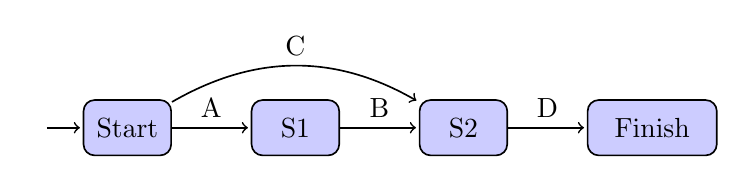
\begin{tikzpicture}[->,shorten >=1pt,auto,column sep=2.2cm,
                    semithick,initial text=]
  \node[initial,block] (s0) {Start};
  \node[block] (s1) [right=of s0] {S1};
  \node[block] (s2) [right=of s1] {S2};
  \node[bw] (s3) [right=of s2] {Finish};

  \path (s0) edge node {A} (s1)
        (s1) edge node {B} (s2)
        (s2) edge node {D} (s3)
        (s0) edge[bend left=30] node {C} (s2);
\end{tikzpicture}
\end{center}

\section*{Data and Task Parallelism}
There are two broad categories of paralellism: data parallelism and
task parallelism. An analogy to data parallelism is hiring a call
center to (incompetently) handle large volumes of support calls,
\emph{all in the same way}. Assembly lines are an analogy to task
parallelism: each worker does a \emph{different} thing.

More precisely, in data parallelism, multiple threads perform the
\emph{same} operation on separate data items. For instance, you have a
big array and want to double all of the elements. Assign part of the
array to each thread. Each thread does the same thing: double array
elements.

In task parallelism, multiple threads perform \emph{different}
operations on separate data items. So you might have a thread that
renders frames and a thread that compresses frames and combines them
into a single movie file.

We'll continue by looking at a number of parallelization patterns,
examples of how to apply them, and situations where they might apply.

\subsection*{Data Parallelism with SIMD}
The ``typical'' boring standard uniprocessor is Single Instruction Single Data (SISD) but since the mid-1980s we've had more options than that. We'll talk about single-instruction multiple-data (SIMD) later on in
this course, but here's a quick look. Each SIMD
instruction operates on an entire vector of data. These instructions
originated with supercomputers in the 70s. More recently, GPUs; the
x86 SSE instructions; the SPARC VIS instructions; and the
Power/PowerPC AltiVec instructions all implement SIMD.

\paragraph{Code.} Let's look at an application of SIMD instructions.

\begin{verbatim}
void vadd(double * restrict a, double * restrict b, int count) {
  for (int i = 0; i < count; i++)
    a[i] += b[i];
}
\end{verbatim}

Compiling this without SIMD on a 32-bit x86 ({\tt gcc -m32 -march=i386 -S}) might give this:
\begin{verbatim}
loop:
  fldl  (%edx)
  faddl (%ecx)
  fstpl (%edx)
  addl  8, %edx
  addl  8, %ecx
  addl  1, %esi
  cmp   %eax, %esi
  jle   loop
\end{verbatim}

We can instead compile to SIMD instructions ({\tt gcc -m32 -march=prescott -mfpmath=sse})
and get something like this:
\begin{verbatim}
loop:
  movupd (%edx),%xmm0
  movupd (%ecx),%xmm1
  addpd  %xmm1,%xmm0
  movpd  %xmm0,(%edx)
  addl   16,%edx
  addl   16,%ecx
  addl   2,%esi
  cmp    %eax,%esi
  jle    loop
\end{verbatim}
The \emph{packed} operations ({\tt p}) operate on multiple data
elements at a time (what kind of parallelism is this?)
The implication is that the loop only needs to loop half as many times.
Also, the instructions themselves are more efficient, because they're
not stack-based x87 instructions.

SIMD is different from the other types of parallelization we're
looking at, since there aren't multiple threads working at once.
It is complementary to using threads, and good for cases
where loops operate over vectors of data. These loops could also be
parallelized; multicore chips can do both, achieving high throughput.
SIMD instructions also work well on small data sets, where thread startup
cost is too high, while registers are just there to use.

We'll see a case study that uses SIMD (also known as vector
instructions) in Lecture 19. In~\cite{lemire18:_multic_simd}, Daniel Lemire argues that vector
instructions are, in general, a more efficient way to parallelize code
than threads. That is, when applicable, they use less overall CPU
resources (cores and power) and can even run faster.


\bibliographystyle{alpha}
\bibliography{459}


\end{document}
